\documentclass[12pt]{article}
\usepackage[letterpaper,top=2cm,bottom=2cm,left=3cm,right=3cm,marginparwidth=1.75cm]{geometry}
\usepackage{graphicx} % Required for inserting images
\usepackage[french]{babel} 
\usepackage[T1]{fontenc}
\usepackage{float} % Pour forcer les images à être là où il faut.
\usepackage{listings} % Listes
\usepackage{color} % Couleurs
\usepackage{xcolor} % Couleurs
\usepackage{lipsum}
\usepackage{amsmath} % Math
\usepackage{amssymb} % Math
\usepackage{amsmath}  % Math
\usepackage{multicol} % Pour les colonnes
\usepackage{hyperref} % Hyperlien
\hypersetup{
    colorlinks=true,
    linkcolor=blue,
    filecolor=magenta,      
    urlcolor=blue,
    pdftitle={Overleaf Example},
    pdfpagemode=FullScreen,
    }
\usepackage{tikz}
\usepackage{pgfplots} % Pour les dessins / formes
\usepackage{siunitx} % Pour formater les unités
\usepackage[
backend=biber,
style=alphabetic,
sorting=ynt
]{biblatex}
\addbibresource{bib.bib} % Bibliographie

% Commandes Math
\newcommand{\K}{\mathbb{K}}
\newcommand{\N}{\mathbb{N}}
\newcommand{\C}{\mathbb{C}}
\newcommand{\R}{\mathbb{R}}
\newcommand{\Rd}{\mathbb{R}^d}
\newcommand{\I}{\mathbf{I}}
\newcommand{\dcrochetg}{[\![}
\newcommand{\dcrochetd}{]\!]}
\newcommand\independent{\protect\mathpalette{\protect\independenT}{\perp}}
\def\independenT#1#2{\mathrel{\rlap{$#1#2$}\mkern2mu{#1#2}}}
\newtheorem{thm1}{Théorème}[section]
\newtheorem{lemme1}[thm1]{Lemme}
\newtheorem{prop1}[thm1]{Proposition}
\newtheorem{rmq1}{Remarque}
\newtheorem{exemple1}{Exemple}
\newtheorem{defin1}{Définition}
% Fin commandes Math

\begin{document}


\begin{titlepage}
    \centering   
    {\huge\bfseries Projet Météorites\par}
    \vspace{1cm}
    {\scshape\Large Rapport de projet tutoré\par}
    \vspace{1.5cm}
    {\large Yannis Petit, Rassem Djimadoum, Duc-Khoi Nguyen \& Garance Malnoë\par
    encadré.e.s par Jean-François Coeurjolly\par}
    \vspace{0.5cm}
    {\large Master 1 SSD\par}
    \vspace{0.5cm}
    {\large Janvier - Avril 2025\par}
    \vspace{3cm}
\end{titlepage}
\pagenumbering{gobble}
\tableofcontents
\clearpage
\pagenumbering{arabic}
\section{Introduction}
Ce rapport présente le projet tutoré réalisé de janvier à avril 2025 dans le cadre de notre première année de Master Statistique et Sciences des Données, sous la direction de Jean-François Coeurjolly. Ce projet porte sur l'analyse du jeu de données \textit{Meteorite Landings} rescencant des météorites tombées au sol. Ce jeu de données est mis à disposition par la Meteoritical Society et accessible sur  l'\href{https://data.nasa.gov/Space-Science/Meteorite-Landings/gh4g-9sfh/about_data}{\underline{Open Data de la NASA}}.\\
\\
En commençant, nous n'avions pas d'objectif défini pour ce projet, l'idée première était d'explorer librement le jeu de données et d'identifier les axes d'analyses les plus pertinents. Toutefois, plusieurs pistes nous avaient été suggérées lors de notre premier échange avec Jean-François Coeurjolly :\\
\begin{itemize}
	\item[-] Étudier la dimension temporelle des données, notamment la présence d'une saisonnalité ou d'une tendance.\\
	\item[-] Analyser les relations entre différentes variables du jeu de données, en particulier l'influence de la masse des 		météorites.\\
	\item[-] Construire un modèle prédictif du nombre de météorites tombées dans un pays en fonction de sa superficie et de sa localisation géographique.\\
	\item[-] Réaliser une étude spatiale afin de determiner si certaines régions sont plus touchées et le cas échéant essayer de déterminer la source des différences.\\
	\item[-] Visualiser les chutes de météorites sur un planisphère.\\
\end{itemize}

Cependant, à cause de la nature des données, nous n'avons pas pu explorer toutes ces pistes. Néanmoins, nous avons pu explorer de nouvelles pistes d'analyse et de modélisation.\\
\\
Nous débutons ce rapport par une présentation de notre organisation de travail ainsi que des outils, langages et bibliothèques utilisés. Nous poursuivons avec une analyse exploratoire des données, comprenant des analyse univariées et multivariées, qui nous ont amener à discuter des pistes à explorer. Ensuite, nous étudions la modélisation des chutes de météorites à l'aide des processus ponctuels, avant de proposer une visualisation interactive du jeu de données sur un globe. Enfin, nous concluons par une réflexion sur l'impact environnemental du projet.\\
\newpage
\section{Organisation, Outils, bibliothèques R et Python}
Organisation : rendez-vous avec Jean-François, répartition du travail, cours de gestion de projet (mermaid chart, plannification).\\
\\
Outils : GitHub, Python, R, VSCode, RStudio. Expliquer que l'on a travaillé en R et en Python parce qu'on est à 4 sur le projet, qu'on maitrise tous les quatre les 2 langages et que l'on a profité des avantages et libraires proposées par les 2 langages.Python pour l'exploration du jeu de données et la modélisation de Rassem parce que package déjà proposés. R pour la visualisation end 3D car package et possibilité de faire une application Shiny.\\
\\
Packages Python : numpy, pandas, geopandas, plotly, shapely.\\
\\
Packages R : ggplot2.\\ 
\\

\section{Exploration des données}
{\setlength{\baselineskip}{1\baselineskip}
L'analyse exploratoire des données a été la première étape de notre projet. Notre but était de comprendre les distributions des varaibles de manière inviduelle mais aussi de trouver et de comprendre les éventuels liens entre variables afin de choisir des axes d'exploration pertinents pour la suite du projet.\\
\\
Pour réaliser les analyses univariées et multivariées, nous avons utilisé Python avec les packages numpy, pandas, geopandas, plotly et shapely et certains visuels ont ensuite été refait en R. Le code se trouve sur le fichier \textit{exploration.ipynb} disponible sur le GitHub.\\
\\
Le jeu de données est composé de 45716 entrées décrites par neuf variables :\\
}

{\setlength{\baselineskip}{1.5\baselineskip}
\begin{itemize}
\item[-] \textbf{name} (qualitative nominale): le nom de la météorite.
\item[-] \textbf{nametype} (qualitative binaire) : le type d'objet soit "Valid" soit "Relict", Relict signifiant qu'il s'agit d'un objet très déformé considéré comme probablement d'origine météorite.
\item[-] \textbf{recclass} (qualitative nominale) : la classe de la météorite (ex : L5, H6, L5, ...).
\item[-] \textbf{mass} (quantitative continue) : la masse de la météorite en grammes.
\item[-] \textbf{fall} (qualitative binaire) : la nature de l'observation soit si la chute de la météorite a été observée (fell) ou si elle a été trouvée au sol (found).
\item[-] \textbf{year} (quantitative continue) : l'année où la météorite a été rescencée.
\item[-] \textbf{reclat} (quantitative continue) : latitude où la météorite a été trouvée.
\item[-] \textbf{reclong} (quantitative continue) : longitude où la météorite a été trouvée.
\item[-]\textbf{geoLocation} : le couple de la latitude et de la longitude.\\
\end{itemize}
}

\subsection{Analyses univariées}
Nous avons commencé par l'analyse univariée de chaque variable en regroupant l'analyse des varaibles \textbf{reclat}, \textbf{reclong} et \textbf{geoLocation}. 
\\
\subsubsection*{Name}
Il n'y a pas de données manquantes pour le nom des météorites et tous les noms sont uniques. Par curiosité, nous avons regardé la répartition du choix de la première lettre :
\begin{figure}[H]
\centering
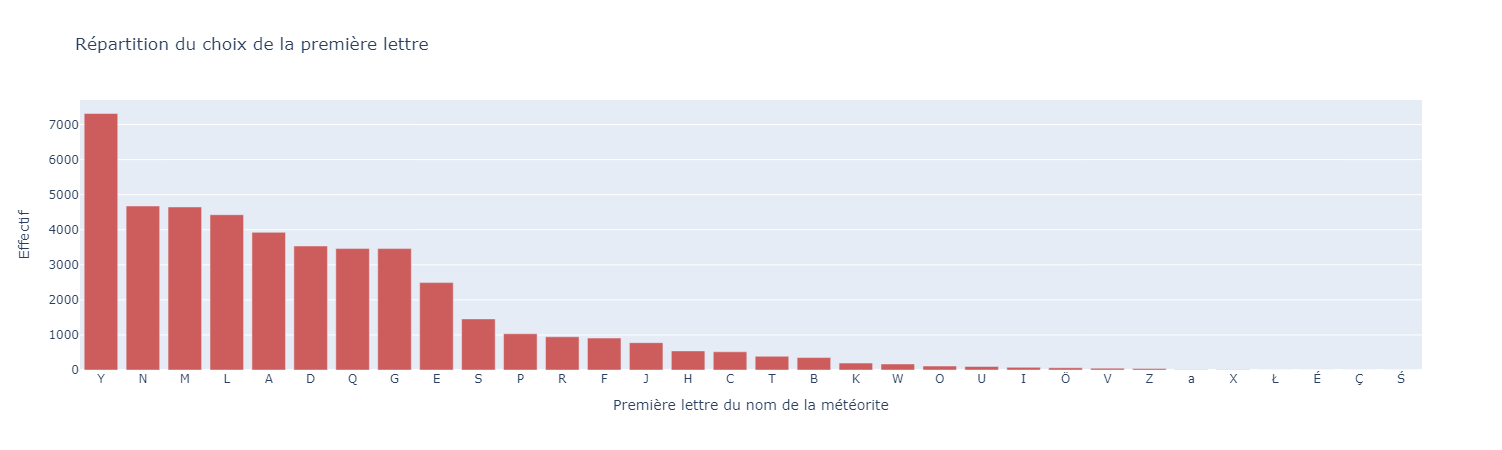
\includegraphics[width=15cm]{Images/exploration/name_barplot_lettres.png}
\caption{Diagramme en barres du choix de la première lettre du nom des météorites}
\end{figure}
Nous pouvons notamment voir que la lettre Y ressort nettement plus souvent que les autres. Cela n'est pas une coincidence mais est lié aux conventions de nommage des météorites [\href{https://www.lpi.usra.edu/meteor/docs/nc-guidelines-2015-february.htm}{source}] : la grande majorité des météorites sont nommées d'après la localité géographique où elles ont été trouvées avec éventuellement une référence numérique après le nom si de nombreuses météorites sont collectées dans la zone. La popularité de la lettre Y est liée aux nombreuses expéditions japonaises effectuées sur le glacier Yamato en Antartique dont les météorites tiennent leur nom. Sur les 7315 météorites dont le nom commence par la lettre Y, 7269 ont été répertoriées sur le glacier Yamato. De même pour la lettre N, sur 4667 météorites, 4499 météorites commencent par "Northwest Africa".
\subsubsection*{Nametype}
Cette variable n'a pas de données manquantes. Comme expliqué précédemment, c'est une variable qualitative binaire décrivant si la météorite a bien été identifiée comme valide (Valid) ou s'il s'agit d'un objet fortement déformé qui est probablement d'origine météorite (Relict). Une large majorité de entrées du jeu de données sont considéréees comme valides : 45641 météorites valides soit 99,8\% contre 75 "Relict" soit 0,02\%.
\subsubsection*{Recclass}
Il n'y a pas de données manquantes pour la variable \textbf{recclass} qui correspond à la classification de la météorite. Le jeu de données compte 422 classes différentes mais les classes L5, L6, H5, H6, LL5 et LL6 sont nettement majoritaires et représente près de 74\% du jeu de données.
\begin{figure}[H]
\centering
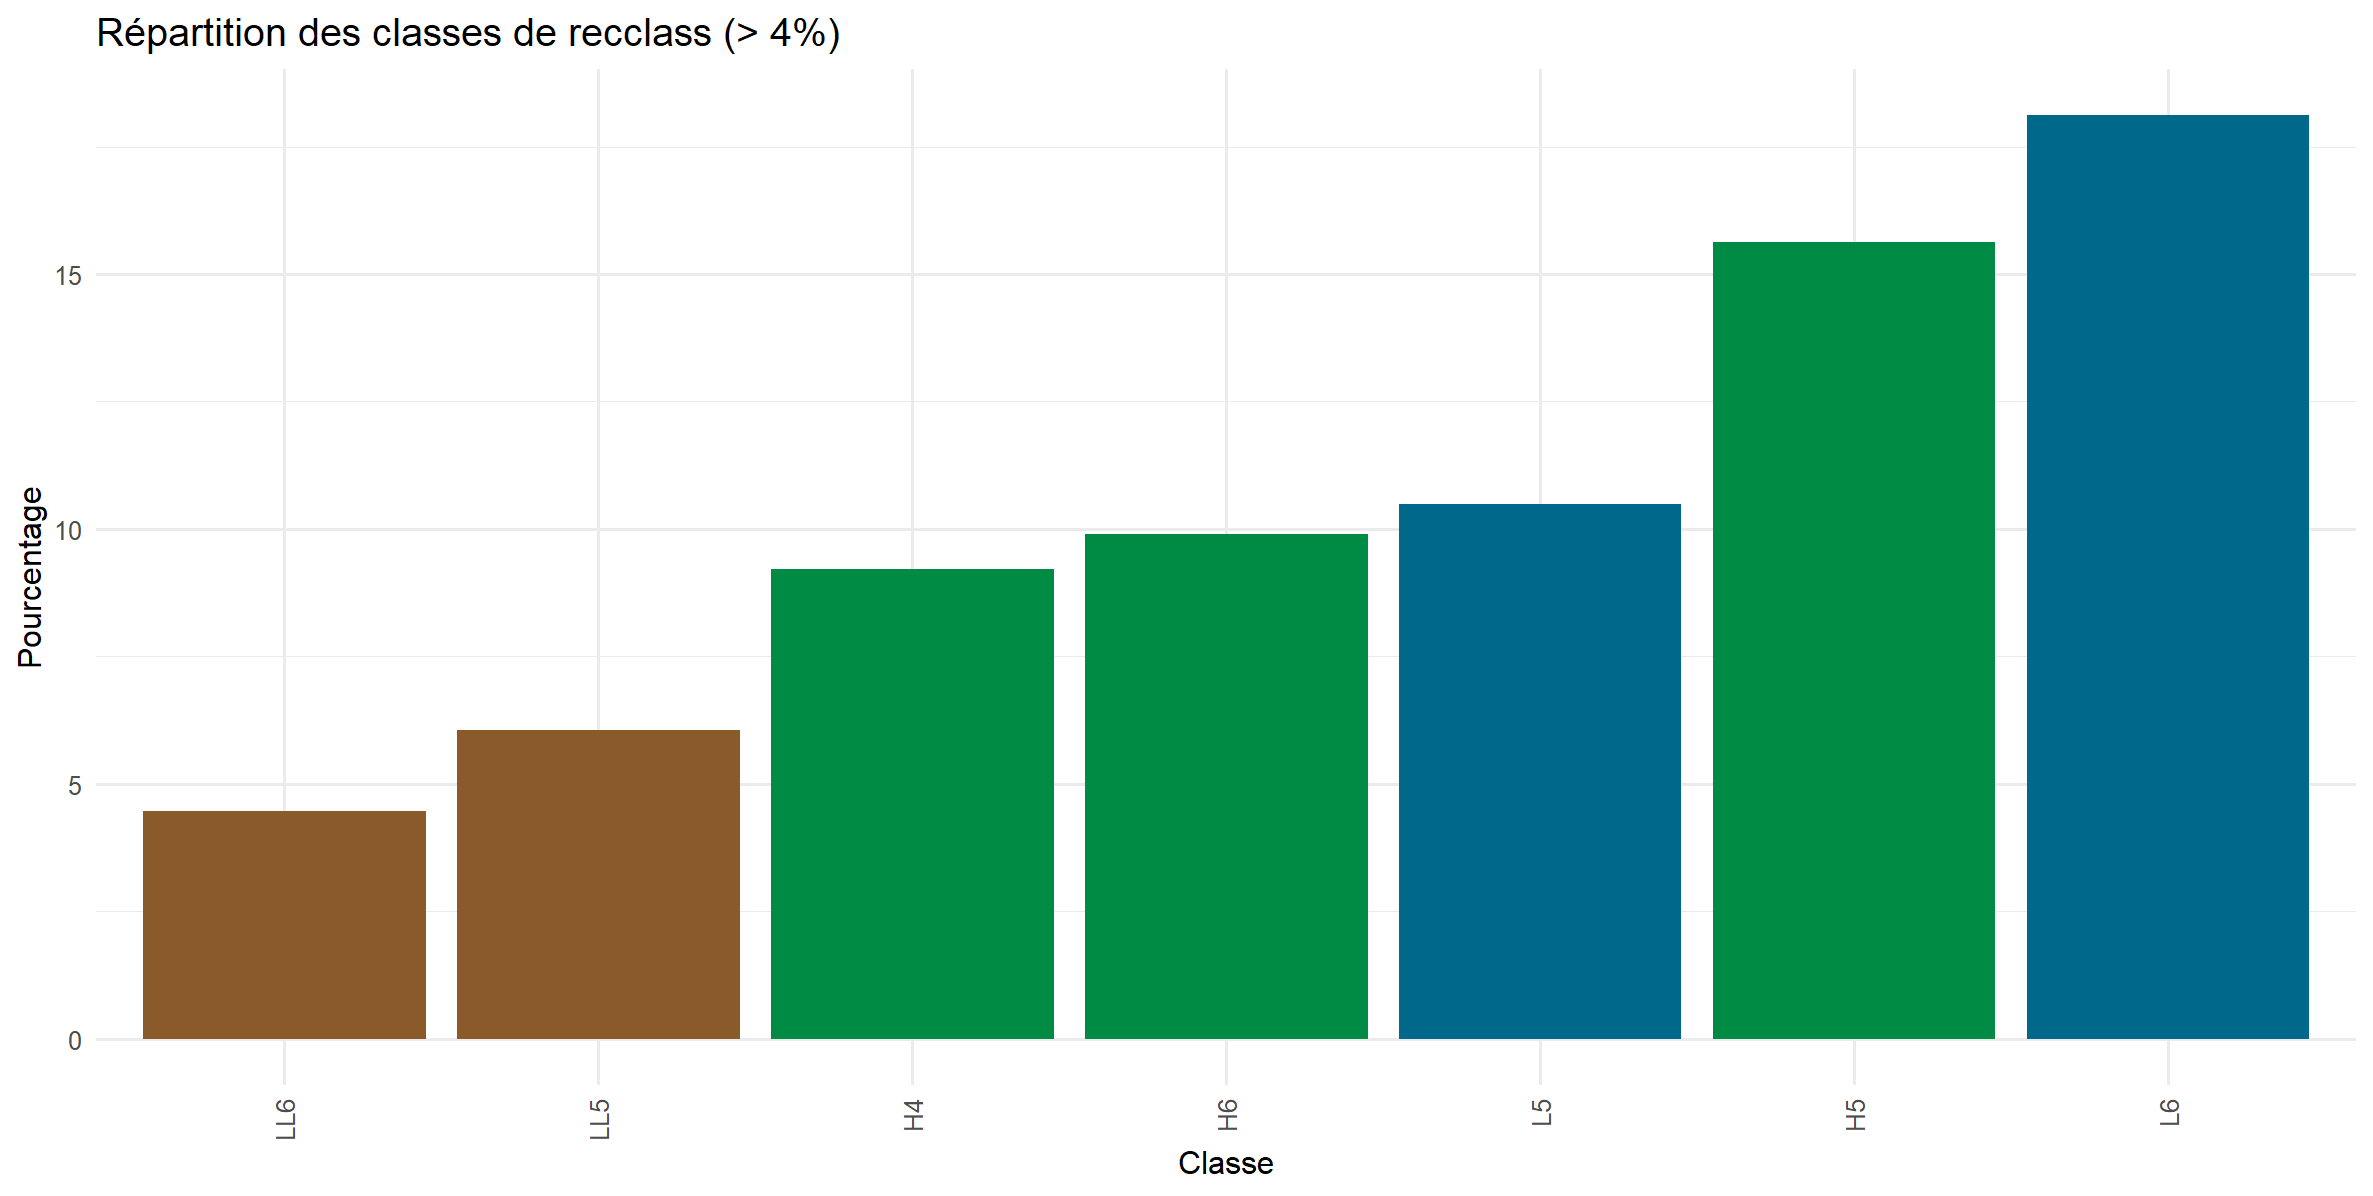
\includegraphics[width=15cm]{Images/exploration/recclass_piechart_class.png}
\caption{Piechart des classes de météorites}
\end{figure}
Ces 6 classes sont celles de chondrites ordinaires [\href{http://www.meteorite.fr/en/classification/}{source}]. Les lettres L, H et LL correspondent aux trois sous-groupes de chrondrites ordinaires : H pour "High Iron" pour celles contenant 25-30\% de fer et de métal libre, L pour "Low Iron" pour celles contenant 20-25\% de fer et moins de métal libre et LL pour celles contenant encore moins de fer ( environ 15-20\%) et très peu de métal libre. Le numéro qui suit correspond au degré de métamorphisme, compris entre 3 et 7, il indique le niveau des modifications subies par la météorites lors de sa chute dues à la pression et la chaleur modifiant leur composition minéralogique, plus le numéro est élevé plus l'alteration est importante.
\subsubsection*{Mass}
Il manque 131 données pour la variable \textbf{Mass} soit moins de 0,3\% du jeu de données. L'analyse de cette variable révèle tout d'abord de grosses différences : plusieurs milliers de météorites pèsent moins de cinq grammes tandis que la plus grosse pèse 60 tonnes.\\
\\
\\
\begin{tikzpicture}

% Dessiner la boîte (boxplot) - proportions arbitraires
\draw[thick] (1, 0) rectangle (8, 2); % Boîte du boxplot

% Médiane (ligne à l'intérieur de la boîte)
\draw[thick] (4.5, 0) -- (4.5, 2); % Ligne médiane

% Moustaches (whiskers)
\draw[thick] (0, 0) -- (0, 2); % Moustache gauche
\draw[thick] (10, 0) -- (10, 2);
\draw[thick] (14.5, 0) -- (14.5, 2); % Moustache droite

%Lignes horizontales
\draw[thick] (0,1) -- (1,1);
\draw[thick] (8,1)--(9,1);
\draw[dashed] (9,1)--(14,1);
\draw[thick] (14,1)--(14.5,1);

% Ajouter des textes en dessous du boxplot
\node at (0, -0.5) {Min};
\node at (1,-0.5) {Q1};
\node at (4.5, -0.5) {Médiane};
\node at (8,-0.5) {Q3};
\node at (10, -0.5) {Moyenne};
\node at (14, -0.5) {Max};

\node at (0, -1) {0};
\node at (1,-1) {7,2g};
\node at (4.5, -1) {32,6g};
\node at (8,-1) {202,6g};
\node at (10, -1) {13,3kg};
\node at (14, -1) {60 tonnes};


\end{tikzpicture}
\\
\\
Près de 75\% des météorites pèsent moins de 200 grammes mais la moyenne est à 13kg, la large majorité des météorites rescencées sont très légères mais le jeu de données rescence quelques très grosses météorites 1388 météorites font plus de 10kg soit environ 3\% du jeu de données. Cela est lié au fait que lors de leur chute les météorites se vaporisent et se fragmentent sous l'effet de la pression et de la chaleur et elles peuvent également se fragmenter à nouveau lors de l'impact. De plus, en réalité, la proportion de petites météorites est sûrement encore plus importantes puisque les grosses météorites ont plus de chances d'être découvertes tandis que les petites météorites passent inapercue et peuvent être confondues avec des roches terrestres ensuite.
\subsubsection*{Fall}
Il n'y a pas de données manquantes pour cette variable. La très large majorité des météorites ont été trouvées (Found), elles représentent 97,5\% du jeu de données.
\subsubsection*{Year}
Pour cette variable, on compte 291 entrée manquantes ainsi qu'une donnée abérrante d'une météorites répertoriée comme tombée en 2101 que nous excluons de l'analyse.\\
\\
Comme pour la variable \textbf{Mass}, il y a de grandes disparités dans la distribution des valeurs :\\
\\
\\
\begin{tikzpicture}

% Dessiner la boîte (boxplot) - proportions arbitraires
\draw[thick] (7, 0) rectangle (12, 2); % Boîte du boxplot

% Médiane (ligne à l'intérieur de la boîte)
\draw[thick] (9.5, 0) -- (9.5, 2); % Ligne médiane

% Moustaches (whiskers)
\draw[thick] (0, 0) -- (0, 2); % Moustache gauche
\draw[thick] (14.5, 0) -- (14.5, 2); % Moustache droite

%Lignes horizontales
\draw[thick] (0,1) -- (2,1);
\draw[dashed] (2,1) -- (5,1);
\draw[thick] (5,1) -- (7,1);
\draw[thick] (12,1) -- (14.5,1);

% Ajouter des textes en dessous du boxplot
\node at (0, -0.5) {Min};
\node at (7,-0.5) {Q1};
\node at (9.5, -0.5) {Médiane};
\node at (12,-0.5) {Q3};
\node at (14, -0.5) {Max};

\node at (0, -1) {860};
\node at (7,-1) {1987};
\node at (9.5, -1) {1998};
\node at (12,-1) {2003};
\node at (14, -1) {2013};


\end{tikzpicture}
\\
\\
Nous pouvons tout de suite voir que la majorité des valeurs sont très récentes : même si le jeu de données contient des météorites datant du IXème siècle, plus de 75\% des météorites des rescencées ont moins de 50 ans. Cependant, cette variable nous permet de nous rendre compte que le jeu de données n'est pas récent puisque la dernière météorite rescencée date de 2013 bien que d'autres météorites soient tombées sur Terre et aient été trouvées.\\
\\
Nous nous sommes alors intéressés plus précisément aux 50 dernières années du jeu de données (1963-2013) :\\
\begin{figure}[H]
\centering
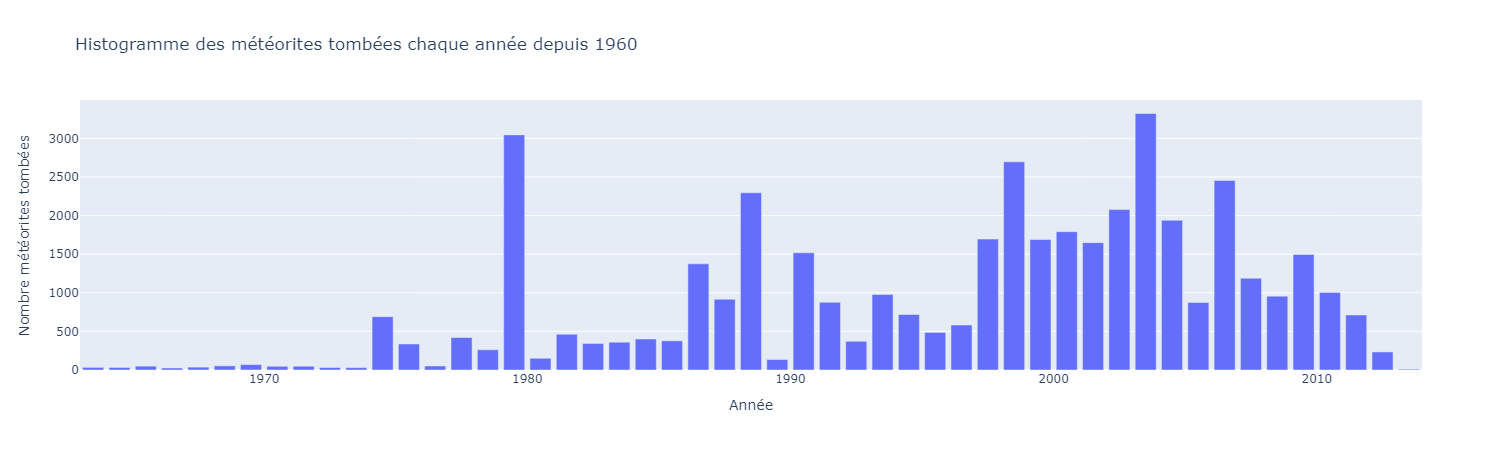
\includegraphics[width=14cm]{Images/exploration/histogramme1963-2013.png}
\caption{Répartition des météorites tombées entre 1963 et 2013}
\end{figure}
Nous observons une nette augmentation du nombre de météorites rescencées à partir de 1974. Nous pouvons alors nous poser la question de la source de l'absence de données dans les années précédentes : est-ce que réellement peu de météorites sont tombées ou n'ont-elles juste pas été référencées ? Avant les années 1970 la détection de météorites reposaient principalement sur des découvertes fortuites ou des témoignages. Les années 1970 ont vu l'essor des réseaux de surveillance qui ont permis un suivi plus rigoureux des météorites comme le \href{https://onlinelibrary.wiley.com/doi/abs/10.1111/j.1945-5100.1989.tb00959.x}{\textit{Meteorite Observation and Recovery Projet}} lancé au Canada en 1974 ainsi que la mise en place de bases de données centralisées comme celle de la \href{https://www.lpi.usra.edu/meteor/metbull.php}{\textit{Meteoritical Society}} et de missions de recherche comme le programme \href{https://caslabs.case.edu/ansmet/faqs/}{\textit{The Antarctic Search for Meteorites}} lancé au milieu des années 1970. Ainsi, l'hypothèse que les météorites n'étaient pas correctement rescencées avant les années 1970 semble plus raisonnable.

\subsubsection*{Location}
Cette variable est celle avec le plus de données manquantes : 7315 entrées où il manque à chaque fois à la fois la longitude, la latitude et la geolocation soit environ 16\% du jeu de données.\\
\\
Dans un premier temps, nous pouvons visualiser sur le planisphère où sont les météorites répertoriées :\\
\begin{figure}[H]
\centering
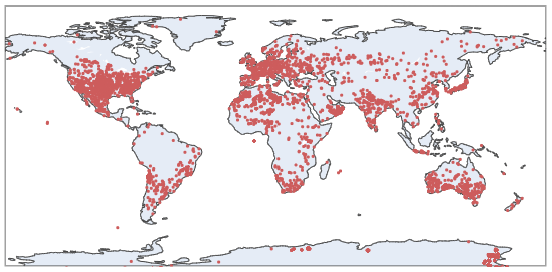
\includegraphics[width=14cm]{Images/exploration/points_monde.png}
\caption{Emplacement des météorites}
\end{figure}
Nous pouvons observer que certaines régions, comme les États-Unis, l’Europe de l’Ouest, le Japon, l’Afrique du Nord et le sud de l’Australie, concentrent une grande partie des recensements. À l’inverse, d’autres zones, telles que le nord du Canada, la Russie ou la forêt amazonienne, sont presque dépourvues de données. Sans surprise, les zones maritimes sont totalement absentes de notre jeu de données, puisqu’il ne répertorie que les météorites tombées sur des terres émergées.\\
\\
Cette répartition inégale met en évidence un biais de recensement important : les régions à faible densité de population, comme la forêt amazonienne ou les territoires du nord du Canada, comptent peu ou pas d’observations, contrairement aux zones fortement peuplées, comme l’Europe de l’Ouest, où les découvertes sont bien plus fréquentes. La seule exception notable à cette tendance est l’Antarctique, où de nombreux recensements ont été réalisés. Cette spécificité s’explique par les nombreuses missions de recherche dédiées à l’étude des météorites dans cette région [\href{https://caslabs.case.edu/ansmet/faqs/}{\textit{source}}]. En effet, les déserts glacées de l’Antarctique représentent des conditions idéales pour l’identification des météorites, facilitant leur repérage et leur collecte.\\
\\
Nous pouvons compléter cette première étude par une étude séparée des longitudes et latitudes :\\
\\
\begin{figure}[H]
\centering
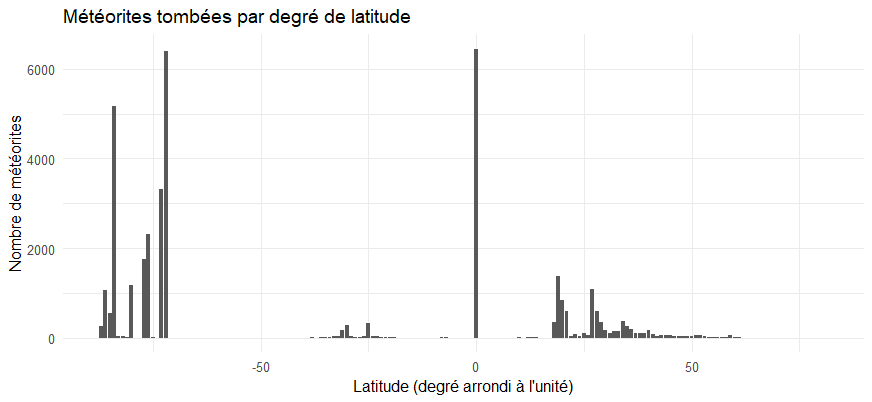
\includegraphics[width=17cm]{Images/exploration/histogramme_latitude.png}
\caption{Latitude des météorites}
\end{figure}
\begin{figure}[H]
\centering
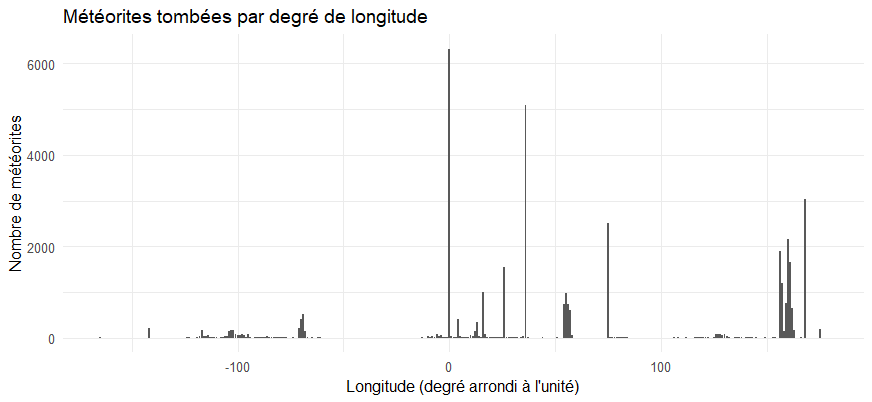
\includegraphics[width=17cm]{Images/exploration/histogramme_longitude.png}
\caption{Longitutde des météorites}
\end{figure}
L'histogramme des latitudes montre une distribution inégale avec plusieurs tendances marquées. On observe un nombre particulièrement élevé d'impacts aux latitudes inférieures à -70°, correspondant aux nombreux points recencés en Antarctique. Un autre pic notable apparaît autour de 0°, ce qui pourrait être associé à l'Afrique du Nord. En revanche, la répartition est plus diffuse entre 15° et 60° Nord, couvrant des régions comme l'Europe de l'Ouest et l'Amérique du Nord.\\
\\
L'analyse des longitudes révèle également une répartition très hétérogène. Une grande partie des météorites enregistrées sont tombées sur des terres émergées, ce qui s'explique par la difficulté de recenser les impacts en milieu océanique. Un pic marqué est visible autour de 0°, correspondant notamment à l'Europe de l'Ouest et au nord de l'Afrique. D'autres concentrations apparaissent entre -150° et -162°, suggérant une fréquence plus élevée d'impacts en Australie et en Antarctique.\\
\\
Nous avons ensuite analysé la répartition du nombre de météorites par pays :
\begin{figure}[H]
 \centering 
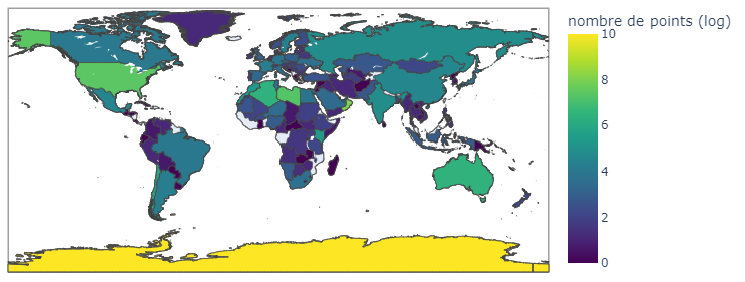
\includegraphics[width=17cm]{Images/exploration/map_points_countries_avec_echelle.png}
 \caption{Nombre de météorites recensées par pays}
 \end{figure}
Sans surprise, l’Antarctique est le territoire où le plus grand nombre de météorites a été recensé, suivi notamment des États-Unis, de la Libye, d’Oman, de l’Australie et de l’Algérie. Cependant, la taille des pays varie considérablement (par exemple, l’Australie et Oman ont des superficies très différentes), ce qui peut biaiser l’interprétation des résultats. Afin de mieux appréhender cette distribution, nous avons calculé le nombre de météorites rapporté à la superficie du pays en km² :
\begin{figure}[H] 
\centering
 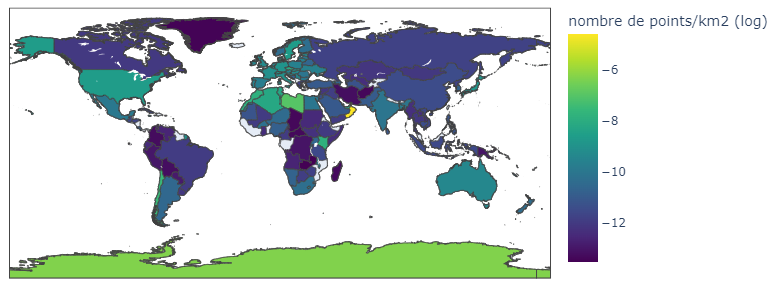
\includegraphics[width=17cm]{Images/exploration/map_points_km2_avec_echelle.png}
 \caption{Densité de météorites recensées par km² et par pays}
 \end{figure}
Cette nouvelle représentation met en évidence plusieurs tendances intéressantes : Oman ressort davantage que dans la carte précédente, tandis que l’Australie et l’Antarctique, bien qu’ayant un grand nombre de météorites recensées en valeur absolue, apparaissent moins dominantes lorsqu’on tient compte de leur superficie. Par ailleurs, les pays d’Europe de l’Ouest présentent des valeurs comparables à celles des États-Unis et des pays d’Afrique du Nord-Ouest.\\
\\
Enfin, nous avons également regardé la répartition des météorites dans le monde selon la masse mais aucune tendance n'est resortie.

\subsection{Analyses multivariées}
\subsubsection*{Analyse quali-quali}
\begin{table}[H]
\centering
\begin{tabular}{rlr}
  \hline
 & Variables & p\_value \\ 
  \hline
1 & nametype - recclass & < $2\times 10^{-16}$  \\ 
  2 & nametype - fall & 0.9085 \\ 
  3 & recclass - fall & < $2\times 10^{-16}$  \\ 
   \hline
\end{tabular}
\end{table}
\subsubsection*{Analyse quanti-quanti}
\begin{table}[H]
\centering
\begin{tabular}{rlrrrr}
  \hline
 & term & mass..g. & year & reclat & reclong \\ 
  \hline
1 & mass..g. &  & -0.1219 & 0.0292 & -0.0219 \\ 
  2 & year & -0.1219 &  & -0.1050 & 0.0903 \\ 
  3 & reclat & 0.0292 & -0.1050 &  & -0.5932 \\ 
  4 & reclong & -0.0219 & 0.0903 & -0.5932 &  \\ 
   \hline
\end{tabular}
\end{table}
\subsubsection*{Analyse quanti-quali}
Nous avons effectué un test de normalité par le test de Shapiro-Wilk qui était très significatif (p-valeur < $2\times 10^{-16}$) donc on effectue le test de Kruskal-Wallis ou de Mann-Whitney qui sont robustes à l'absence de l'hypothèse de normalité. O
\begin{table}[H]
\centering
\begin{tabular}{rllr}
  \hline
 & Variable quantitative & Variable qualitative & p-value \\ 
  \hline
1 & mass..g. & nametype & < $2\times 10^{-16}$ \\ 
  2 & year & nametype &< $2\times 10^{-16}$  \\ 
  3 & reclat & nametype &< $2\times 10^{-16}$ \\ 
  4 & reclong & nametype & 0.1026 \\ 
  5 & mass..g. & recclass & < $2\times 10^{-16}$  \\ 
  6 & year & recclass & < $2\times 10^{-16}$  \\ 
  7 & reclat & recclass & < $2\times 10^{-16}$  \\ 
  8 & reclong & recclass & < $2\times 10^{-16}$  \\ 
  9 & mass..g. & fall &< $2\times 10^{-16}$  \\ 
  10 & year & fall & < $2\times 10^{-16}$  \\ 
  11 & reclat & fall &< $2\times 10^{-16}$  \\ 
  12 & reclong & fall &< $2\times 10^{-16}$  \\ 
   \hline
\end{tabular}
\end{table}

\subsection{Discussion des limites du jeu de données}

L’étude des données manquantes a révélé que seules trois variables sont concernées : la masse des météorites, l’année de leur chute et leur localisation. Malgré ces lacunes, en supprimant toutes les entrées comportant au moins une valeur manquante, il reste 38 115 observations, soit environ 83\% du jeu de données initial. Ce volume semble suffisant pour mener des analyses pertinentes.\\
\\
L’analyse univariée des variables, en particulier l’emplacement et l’année de chute, a mis en évidence plusieurs biais significatifs dans les données. D’une part, un biais temporel est présent : les météorites récentes sont surreprésentées en raison de l’amélioration du suivi, de la centralisation des bases de données et du développement de missions dédiées à leur recherche. D’autre part, un biais géographique est également perceptible : les météorites sont davantage recensées dans les zones densément peuplées, à l’exception notable de l’Antarctique, où des campagnes de recherche intensives ont été menées. Enfin, il est probable qu’un biais en faveur des météorites les plus massives existe, celles-ci étant plus faciles à identifier et à distinguer des roches environnantes. Il est donc évident que toutes les météorites ne sont pas répertoriées.\\
\\
Un problème majeur réside dans le manque d’informations sur la constitution du jeu de données : le site de la NASA où nous avons récupéré nos données (ainsi que d’autres sources en ligne) ne précise pas si les données proviennent uniquement d’observations scientifiques (téléscopes, chercheurs) ou si elles incluent des signalements grand public. Cette incertitude complique l’interprétation des analyses.\\
\\
Concernant les pistes que nous souhaitions initialement explorer, plusieurs ont dû être écartées :
\\
 - Analyse temporelle : Cette approche s’est révélée impraticable pour plusieurs raisons. Tout d’abord, les données disponibles ne contiennent que l’année de chute des météorites, sans précision sur le mois ou le jour. De plus, le biais temporel implique que seules les quarante dernières années sont véritablement exploitables, une période trop courte pour une analyse robuste. Nous avons tenté d’explorer un autre jeu de données, MetCat, qui inclut des informations plus détaillées sur la temporalité (mois, jour). Cependant, son utilisation s’est avérée problématique : la précision temporelle reste insuffisante (mois indiqués sous des catégories larges comme Printemps ou Juin-Août), et le nombre d’observations réellement exploitables est trop faible en raison de la rareté des données bien documentées. Cette piste a donc été abandonnée.\\
\\
- Modélisation prédictive : Construire un modèle visant à prédire le nombre de météorites tombées dans un pays en fonction de sa superficie et de sa position géographique n’a pas été jugé pertinent. En effet, la présence d’un fort biais de recensement fausse la relation entre ces variables et le nombre de météorites réellement observé.\\
\\
Finalement, nous avons décidé de nous concentrer sur deux axes principaux :\\
\\
- Une visualisation en 3D, afin de pallier les distorsions engendrées par la projection plane du planisphère et d’obtenir une représentation plus fidèle de la répartition des météorites.\\
\\
- Une analyse du processus sous-jacent à la chute des météorites, en testant si leur distribution suit un processus ponctuel (c’est-à-dire aléatoire), notamment via l’application d’un processus de Poisson homogène et inhomogène, complété par des simulations.

\section{Modélisation de processus ponctuels}
Math processus de Poisson homogène et inhomogène + simulations de Rassem.\\
\\
K de Ripley.\\
\section{Visualisation en 3 dimensions}
Travail de Yanis et Duc-Khoi.

Capture d'écran des possibilités de visualisation que nous proposons + lien vers une page hébergeant l'application shiny ?

\section{Conclusion}
\section{Remerciements}
\cite{these_remi_coulaud}
\section{Références}
\printbibliography
- Lien vers l'article sur les météorites en Antartique.
\section{Impact environnemental et sociétal du projet}
J'ai remis les consignes du pdf de l'Ensimag. Cette section doit représenter envrion 20\% du rapport.
\subsection{Impact environnemental personnel}
Partie moins importante.
Estimation de l'impact des trajets domicile-travail, impact de la consommation des équipements utiliés (ordinateurs perso/fixes, temps d'utilisation des serveurs github,...), autres impacts.
Expression en exprimé en kg eq. CO2.

\subsection{Impact global du projet}
Dans cette section, nous vous demandons d’évaluer l’impact global du projet sur lequel vous avez travaillé. Si vous avez travaillé sur un produit fini (logiciel, infrastructure…), vous devrez mettre en valeur non seulement l’impact du produit lui-même mais également l’évolution de cet impact entre le début et la fin de votre PFE. Si vous avez travaillé sur une preuve de concept, un avant-projet, un projet de recherche et développement ou un projet de recherche pure, votre évaluation devra tenir compte des possibles utilisations de votre travail dans un contexte applicatif. Cette section sera la plus importante de la partie consacrée à l’impact environnemental et sociétal. Nous ne vous demandons pas une simple évaluation technique, mais une véritable réflexion déclinée sur deux plans :
1. à petite échelle (concernant uniquement votre projet, à court terme)
2. à plus grande échelle (long terme, et dans l’hypothèse où le même type de projet venait à se généraliser et/ou
se transposer dans différents secteurs)
Nous demandons dans cette section un avis honnête, critique et argumenté sur les impacts positifs et négatifs du projet. Vous ne serez pas évalué sur la quantité ni la qualité des bonnes pratiques sociales et environnementales mises en œuvre dans le cadre de votre PFE : il est donc inutile d’écoblanchir votre discours. Ce qui nous importe est la vision critique que vous adoptez.

\subsection{Politique de la structure d'acceuil}
Dans cette section, nous vous demandons de dresser une liste des actions menées par la structure d’accueil sur les aspects écologiques et sociaux. Cela peut concerner des actions individuelles ou la mise en œuvre d’une véritable politique dans ce domaine. De même, cela concerne à la fois des politiques extérieures éventuelles (fondations, dons à des organismes…), mais également des actions destinées à l’ensemble des collaborateurs de l’entreprise (conditions de travail, mise en œuvre de bonnes pratiques environnementales au quotidien…). Vous mettrez bien entendu en évidence tous les aspects positifs de cette politique. En revanche, si vous estimez qu’il y a des voies d’amélioration possibles en termes de politique de responsabilité sociale et environnementale, nous vous encourageons à proposer une liste d’actions concrètes qui pourraient être mises en œuvre. Cela montrera non seulement votre capacité à réaliser une analyse critique, mais cela vous permettra également d’être une force de proposition pour votre structure d’accueil.
\newpage
\section{Annexe}


\end{document}